\documentclass{article}


\usepackage{PRIMEarxiv}

\usepackage[utf8]{inputenc} % allow utf-8 input
\usepackage[T1]{fontenc}    % use 8-bit T1 fonts
\usepackage{hyperref}       % hyperlinks
\usepackage{url}            % simple URL typesetting
\usepackage{booktabs}       % professional-quality tables
\usepackage{amsfonts}       % blackboard math symbols
\usepackage{nicefrac}       % compact symbols for 1/2, etc.
\usepackage{microtype}      % microtypography
\usepackage{lipsum}
\usepackage{fancyhdr}       % header
\usepackage{graphicx}       % graphics
\graphicspath{{media/}}     % organize your images and other figures under media/ folder

% Review build (brief Section 7): \reviewfalse gives the clean build.
\newif\ifreview
\reviewtrue
\ifdefined\cleanbuild\reviewfalse\fi
% review_setup.tex -- packages needed by Sections 1-3 and the review-build machinery (brief Section 7).
% The switch \ifreview is declared in the main file. \reviewfalse gives the clean build:
% no colour, no margin notes, no banners, no Notes box, no todo notes.

\usepackage[numbers,sort&compress]{natbib}  % \citet/\citep used by the Related Work draft
\usepackage{amsmath,amssymb}
\usepackage{xcolor}
\usepackage{array,tabularx,multirow}
\usepackage[most]{tcolorbox}
\ifreview
  \usepackage[textsize=tiny,color=orange!25,bordercolor=orange!60]{todonotes}
\else
  \usepackage[disable]{todonotes}
\fi

% margin notes need room in the 1in margins of PRIMEarxiv
\AtBeginDocument{\setlength{\marginparwidth}{0.82in}\setlength{\marginparsep}{0.08in}}

\definecolor{revclaim}{RGB}{0,72,186}     % method and claim changes
\definecolor{revword}{RGB}{140,120,170}   % wording fixes that change no claim (lighter)
\definecolor{revdec}{RGB}{196,96,0}       % open decisions D1-D9
\definecolor{revbanner}{RGB}{226,236,250}

% \rev{text}: method or claim change. \revw{text}: wording fix only.
\newcommand{\rev}[1]{\ifreview{\color{revclaim}#1}\else#1\fi}
\newcommand{\revw}[1]{\ifreview{\color{revword}#1}\else#1\fi}
% \revwhy{source}: margin note naming the source of the change (brief / review / v5.1 section, or REF-n).
\newcommand{\revwhy}[1]{\ifreview\leavevmode\marginpar{\raggedright\tiny\sffamily\color{revclaim}#1}\fi}
\newcommand{\revwhyw}[1]{\ifreview\leavevmode\marginpar{\raggedright\tiny\sffamily\color{revword}#1}\fi}
% \revdel{what}: marks a deletion from the baseline text, which colour cannot show.
\newcommand{\revdel}[1]{\ifreview\leavevmode\marginpar{\raggedright\tiny\sffamily\color{red!70!black}deleted: #1}\fi}
% \dec{Dn}{text}: text written with the default of open decision Dn.
\newcommand{\dec}[2]{\ifreview{\color{revdec}#2}\textsuperscript{\tiny\sffamily\color{revdec}[#1]}\else#2\fi}

% Banner at the start of a section written new against the baseline.
\newcommand{\newsectionbanner}[1]{%
  \ifreview
  \begin{tcolorbox}[colback=revbanner,colframe=revclaim!60,boxrule=0.4pt,arc=1pt,left=4pt,right=4pt,top=2pt,bottom=2pt,fontupper=\footnotesize\sffamily]
  \textbf{New section.} #1
  \end{tcolorbox}
  \fi}

% Notes box, first page of the review build only.
\newtcolorbox{reviewnotes}{breakable,enhanced,colback=orange!4,colframe=revdec!70,boxrule=0.5pt,arc=1pt,
  left=5pt,right=5pt,top=3pt,bottom=3pt,fontupper=\scriptsize,title={\sffamily\small Notes for the authors (review build only)},
  fonttitle=\bfseries}

\newcommand{\mask}{\operatorname{mask}}
\newcommand{\EM}{\mathrm{EM}}
\newcommand{\ED}{\mathrm{ED}}


%Header
\pagestyle{fancy}
\thispagestyle{empty}
\rhead{ \textit{ }} 

% Update your Headers here
\fancyhead[LO]{Running Title for Header}
% \fancyhead[RE]{Firstauthor and Secondauthor} % Firstauthor et al. if more than 2 - must use \documentclass[twoside]{article}



  
%% Title
\title{Substitution Artifacts in Shapley-Based Temporal Attribution:
Characterizing and Correcting Masking-Background Bias on
Mean-Nonstationary Time Series
%%%% Cite as
%%%% Update your official citation here when published 
\thanks{\textit{\underline{Citation}}: 
\textbf{Authors. Title. Pages.... DOI:000000/11111.}} 
}

\author{
  Myroslav Mishchuk \\
  Silesian University of Technology \\ 
  Gliwice, Poland \\
  Lviv Polytechnic National University \\ 
  Lviv, Ukraine \\
  \texttt{myroslav.mishchuk@polsl.pl} \\
   \And
  Rafał Cupek \\
  Silesian University of Technology \\ 
  Gliwice, Poland\\
  \texttt{rafal.cupek@polsl.pl} \\
    \And
  Olena Pavliuk \\
  Silesian University of Technology \\ 
  Gliwice, Poland \\
  Lviv Polytechnic National University \\ 
  Lviv, Ukraine \\
  \texttt{olena.pavliuk@polsl.pl} \\
}


\begin{document}
\maketitle

\ifreview% review_notes.tex -- Notes box, review build only (brief Section 7). Mirrors notes/OPEN_DECISIONS.md.
\begin{reviewnotes}
\textbf{How to read this build.} \textcolor{revclaim}{Blue}: method or claim change against the baseline (Related Work); \textcolor{revword}{lilac}: wording fix that changes no claim; margin notes name the source (B\S\ = brief, R\S\ = readiness review, V\S\ = v5.1, P\S\ = style preferences, REF-$n$ = notes/REFERENCES\_AUDIT.md); red margin notes mark deletions. Sections~1 and~3 are new and carry a banner instead of word-level colour. \textcolor{revdec}{Orange}~[D$n$]: text written with the default of an open decision. Orange margin boxes: unverified items. The clean build (\verb|\reviewfalse|) removes all of this.

\medskip\textbf{1. Open decisions (default written in the text).}\\[1pt]
\begin{tabularx}{\linewidth}{@{}l>{\raggedright\arraybackslash}X>{\raggedright\arraybackslash}p{3.2cm}@{}}
D1 & B2c (coalition-conditional TAB) included as a variant of B2. & \S3.4 (B2c), Table~2 \\
D2 & Longer window $L:=96$, from DegradX's declared grid; the ACIIDS sequence length could not be checked (paper not available). & \S3.5, extensions \\
D3 & B1 = per-channel training mean; TimeSHAP's average event (median) as a variant. ``As in ACIIDS Eq.~3'' is unverified. & \S3.4 (B0--B-pristine) \\
D4 & ``mean component'' (not ``level''); v5.1's ``level index'' $\to$ ``state index''. & \S3.1; \S2.1 wording \\
D5 & M-$\psi$ included, marked ``conditional on the pilot''; $\psi$ itself is not specified by any input. & \S3.5, targets and models \\
D6 & Non-Shapley comparators dropped from the design; discussed in Related Work only. & \S2.4 \\
D7 & Primary synthetic architecture = DegradX's LSTM; the attention LSTM only in the case study. & \S3.5, \S3.6 \\
D8 & Threshold $\vartheta$ of the function-identity check left open. The X9 pilot (HUST; IG and occlusion only) fitted to 1--2\,\% of the noise term's SD, with temporal profile error 0.45--0.47 across ten models against a method gap of 0.035 (readiness review \S2.2; unpublished, so not in the text). & \S3.5, M-obs \\
D9 & Target journal EAAI. Not in the text; see conflict C1. & -- \\
\end{tabularx}

\medskip\textbf{2. Method constants that no input fixes} (written as symbols; values needed before the experiments): $K$, bin scheme and minimum count of B2; the running summary $h$, cap $d$ and near-duplicate threshold of the index-channel screen; $t_{\min}$, $\mathcal{M}$, $\omega$, $P$ of B3; architecture and training of the B4 imputer; implementation and hyperparameters of the boosted-tree control; $\psi$; the quantiles that define the near and far bands of M2; the positions $u_0$ swept by M5; the precision of permutation sampling for $\phi^\star_b$; amplitude, period and phase of P-GEN; the subsample fractions of E2; the profile of the cross-estimator check. Chosen here and to be confirmed: the construction of the trended null channel (charge-time mapping, random start, held after the other unit's end of life); M-R ensembles with DegradX's ten-member design; recency weighting only (uniform not run).

\medskip\textbf{3. Unverified items} (\verb|% TODO| in the .bib or \verb|\todo| in the text).
(i) DegradX arXiv identifier unknown. (ii) ACIIDS paper absent from \texttt{./style}: B1 as in its Eq.~3; its sequence length (D2); PCoE cells and preprocessing; attention-LSTM architecture; what the pipeline correction changes; the list of published findings for the case study. Its bibliographic record is verified (Crossref). (iii) TSHAP: only title and abstract accessible; its background-selection rule and its applicability to the LSTM regressor and to cell-level players are unverified (v5.1 \S9 item). (iv) GroupSegment-SHAP is cited in its CIKM~'26 version; the claims were checked against arXiv v2 (2026-08-21), the CIKM text was not accessible. (v) Repository URL of this paper's code. (vi) v5.1 \S9 ``to verify'' list: TimeX now verified (Queen et al., NeurIPS 2023); spurious-regression, Zeiler--Fergus, knee-identification, CRP-detection, C-MAPSS and NARMA references are not used; battery dataset facts are taken from DegradX; arXiv publication status checked 2026-11-03.

\medskip\textbf{4. Conflicts between inputs not resolved.}
C1: the brief names \texttt{elsarticle}; the project is PRIMEarxiv. Template untouched; an EAAI submission needs a port.
C2/C5: the ACIIDS findings quoted in v5.1 (Eq.~3, Spearman 0.078, 16.9\,\% pruning) are not used, since the paper is the only allowed source and is unavailable.
C4: DegradX's README cites it as an ACIIDS~2027 submission; the brief asks for the arXiv entry.
C9: v5.1's B4 validity gate also used fill surprisal, which needs the density model that the brief's instrument set drops; only the held-out imputation error is kept.
Brief \S2.5 does not list P-GEN among the extensions, while \S3 item 8 and E5 require it; it is included as a declared extension.
The brief's ``function-identity gate'' is written as ``function-identity check'' (P\S3.4, plain words); RQ1 and RQ2 omit the labels B0, B1, B-pristine and B4, which are not defined before Section~3 (P\S4.1).
Bibliography style changed from \texttt{unsrt} to \texttt{unsrtnat} and natbib loaded, as the existing \verb|\citet| calls require; outside \S1--\S3 the template's demo section, the lipsum abstract and the conclusion placeholder remain.

\medskip\textbf{5. Novelty re-check} (searches 2026-11-03, after v5.1's 2026-07-19). No candidate provides contribution 2 or 3.
Delta-XAI/SWING (Kim et al., ICLR 2026): past window as Integrated Gradients baseline; classification; no ground truth $\to$ \S2.4.
GRAIL (Menadjiev et al., arXiv:2610.29036): region players with baselines from a conditional generator; ECG classification $\to$ \S2.4.
TempShap (Zhao et al., arXiv:2610.33330): cell-level Shapley for forecasting with the training mean as background $\to$ \S2.5.
Zhang et al.\ (arXiv:2603.05093, v2, retitled): path selected by transport, explicitly no manifold claim $\to$ \S2.2 (moved from \S2.1).
Not added: a synthetic ground-truth framework for images, tabular data and time series (arXiv:2609.30397; no mean-nonstationary regression) and a study of DAG-faithfulness of marginal attribution for time series (arXiv:2607.16236).
\end{reviewnotes}
\fi


\begin{abstract}
\lipsum[1]
\end{abstract}


% keywords can be removed
\keywords{explainable AI \and Shapley values \and temporal attribution \and time series \and mean-nonstationarity \and remaining useful life}


%==============================================================================================
\section{Introduction}
\label{sec:intro}
%==============================================================================================
\newsectionbanner{Written new against the baseline, which held only an RQ list (replaced by the RQs of brief \S2.1). Sources: brief \S2.1--2.2; v5.1 \S1.1--1.4; DegradX \S1 and \S4.4. Open decisions are coloured and tagged [Dn].}

Post-hoc attribution is the explainable artificial intelligence (XAI) approach most frequently applied to models of manufacturing and industrial cyber-physical systems, since it can be applied to a model that is already trained without altering it \citep{moosavi2024explainable}. For sequence models, Shapley-based temporal attribution, which carries SHapley Additive exPlanations (SHAP) \citep{lundberg2017unified} over to sequences \citep{bento2021timeshap}, assigns to each cell of an input window, one channel at one position, a share of the model's output. The share is obtained by removing cells and observing how the output changes. A trained model cannot receive an input with cells missing, however, so removal is simulated by substitution: the removed cells take the values of a background input, and the model is evaluated on the result. How features are removed is one of the respects in which removal-based explanations differ \citep{covert2021explaining}.

The background is left to the user. TimeSHAP describes it as an uninformative input, often taken to be zero or the average feature values of the dataset \citep{bento2021timeshap}. Later temporal Shapley methods note that the effect of background selection remains understudied \citep{nguyen2025tshap} and measure that attributions change when the background changes \citep{kim2026groupsegment, papadeas2026empirical}. The choice matters for a second reason, beyond sensitivity. Shapley values sum to the difference between the model's output on the input and its output on the background \citep{lundberg2017unified, sundararajan2020many}, so the background also fixes which quantity is explained. Different backgrounds therefore answer different questions about the same prediction \citep{merrick2020explanation, mamalakis2023carefully}.

On mean-nonstationary data, whose mean component changes along the sequence, an unconditional background is systematically far from the observations wherever the mean component is far from it. The substituted window then combines values that the process does not produce together, and the model is evaluated outside the support of its training distribution, where its output is an extrapolation \citep{hooker2021unrestricted} and the resulting explanations can be incorrect \citep{frye2021shapley}. For perturbation-based saliency, this effect was observed on synthetic series with a linear trend, on which perturbation methods sampled unlikely or out-of-domain counterfactuals \citep{tonekaboni2020went}. The attribution of a cell thus sums two parts that it does not separate: the information the cell carries, and the model's response to an input it was never trained on. This is the organizing claim of the paper:
\begin{center}
\itshape The explainer assumes stationarity where the model does not.
\end{center}
A sequence model trained on a population of units legitimately reads the mean component, which in degrading systems carries the larger part of the information about the target variable \citep{degradx2026}. An unconditional background treats every position as exchangeable with one substitute, which is a stationarity assumption that the data violate.

Detrending the inputs does not remove the problem. A post-hoc explanation has to explain the model as deployed, and a model trained on detrended inputs is a different model. Detrending at explanation time only, in turn, evaluates the deployed model on inputs unlike its training data, which is the same problem again. Where the mean component carries the target variable, removing it changes the task rather than the explanation.

Substitutes that respect the data exist in two lines of work. In the Shapley framework, conditional value functions keep the evaluations on the data distribution, at the cost of estimating conditional distributions or training a generative model \citep{frye2021shapley, aas2021explaining}, and in images, generative infilling replaces constant patches \citep{chang2019explaining, jain2022missingness}. For time series, perturbation-based saliency methods draw counterfactuals from generators conditioned on the past or learn in-distribution perturbations \citep{tonekaboni2020went, liu2024explaining}. These substitutes come from learned models. None of them uses the structure that mean-nonstationarity itself provides, a low-dimensional state that the unit has reached and on which a substitute can be conditioned without a generative model. Nor could a choice between backgrounds be checked until recently, since attribution ground truth under sustained mean-nonstationarity was not available. DegradX \citep{degradx2026}\todo{DegradX arXiv identifier not yet known (brief \S5.3)} now supplies it at every observation of units generated from profiles fitted to three battery-degradation datasets. Its own results, however, show that this ground truth cannot rank backgrounds on trained models. Ten equally accurate long short-term memory (LSTM) networks \citep{hochreiter1997long} differ more than the attribution methods do in all but one case: in rank agreement, for instance, the methods differ by at most 0.073, whereas each method's range over the ten models is at least 0.099. Switching TimeSHAP's background moved its rank agreement by at most 0.04, and this was enough to change its place among the methods in two of the three profiles \citep{degradx2026}. A comparison of backgrounds scored in this way would be decided by which model happened to be trained.

This paper characterizes how masking backgrounds distort temporal Shapley attributions of models of mean-nonstationary data, proposes trend-aware backgrounds (TAB), which condition the substitute on the state of the unit, and evaluates both. The evaluation replaces the common ground truth with one per background. Models are trained on a target variable that is a known function of the observed window, so that on its data support a trained model reproduces that function. For every background, the exact attribution of the known function under that background is then the ground truth. The difference between the model's attribution and this ground truth is the distortion the background causes, separated from the information the background removes. We address three research questions (RQs):
\begin{itemize}
    \item \textbf{RQ1}: How large and how structured is the distortion that unconditional backgrounds introduce into temporal Shapley attributions of models of mean-nonstationary data?
    \item \textbf{RQ2}: Do trend-aware backgrounds reduce that distortion? How much of the prediction do they still explain, and how do they compare with a learned conditional imputer?
    \item \textbf{RQ3}: Do the distortion signatures found on models of known functions also appear on models of remaining useful life (RUL) trained on generated units, and on models trained on the measured cells of the same datasets?
\end{itemize}
In addition, a two-step case study re-examines, on a corrected pipeline, the findings of the authors' earlier TimeSHAP study of an LSTM model of battery RUL \citep{mishchuk2026explaining}.

The contributions of this paper are as follows:
\begin{itemize}
    \item A taxonomy of substitution artifacts (A1--A6) with one instrument per artifact, measured against exact ground truth.
    \item TAB-state and TAB-traj, two trend-aware backgrounds defined formally for general mean-nonstationarity, each with its assumptions, diagnostics and operating envelope.
    \item An evaluation design for masking backgrounds, built on DegradX, in which a trained model reproduces a known function on its data support, so that the ground truth is exact for every background and the distortion a background causes is separated from the information it removes.
    \item A two-step case study of the authors' published attribution findings, on a corrected pipeline.
\end{itemize}
The mechanism and the backgrounds are stated for mean-nonstationarity in general. The experiments use its monotone instance, in which the mean component follows an irreversible degradation, together with one probe in which it does not; no claim is made beyond that scope. Battery RUL estimation is the flagship application, since the capacity fade of battery cells is the monotone instance in physical form and three public datasets \citep{severson2019data, ma2022real, cui2024data} have calibrated and validated DegradX profiles \citep{degradx2026}. The code and the extensions of the testbed are released with the paper.\todo{Repository URL for this paper's code}


%==============================================================================================
\section{Related Work}
\label{sec:related}
%==============================================================================================

\subsection{The value-function problem in Shapley explanations}
\label{sec:related:offmanifold}

In the Shapley framework, the value of a feature coalition is computed by evaluating the model with the complementary features replaced or marginalized, and the choice of this value function is known to change the resulting explanation. \citet{frye2021shapley} demonstrated that ``off-manifold'' evaluation --- splicing replacement values into an observed instance without regard for feature dependence --- can produce incorrect explanations, and proposed two on-manifold remedies: substitution via a generative model of the data, and directly learning the value function. \citet{aas2021explaining} developed conditional-expectation approximations for dependent features in the kernel-SHAP setting. The conceptual axis along which these proposals differ is now standard: interventional value functions stay true to the model but evaluate it on unrealistic inputs, while observational/conditional value functions respect the data distribution at the cost of attributing importance to merely correlated features \citep{chen2020true, janzing2020feature, sundararajan2020many}. \rev{The same extrapolation makes permute-and-predict importance measures misleading when features are strongly dependent \citep{hooker2021unrestricted}.}\revwhy{B\S5.5 thread 1; cited in \S1 (P\S2.11); REF-9} \citet{yeh2022threading} formalized desiderata spanning both views and showed that both classes are vulnerable to manipulation in low-density regions.\revdel{``The line remains active: recent work casts on-manifold attribution as transport along generative flows''. Source retitled and disclaims manifold membership; reworded in \S2.2 (REF-22)}

Two properties of this literature matter for the present paper. First, its data model is static \rev{(tabular or image data)}\revwhy{REF-8: Frye et al.\ also use images; parenthesis on the moved Zhang et al.\ sentence deleted}: the manifold is generic, and the proposed remedies therefore require estimating conditional distributions or training generative surrogates. Second, none of it examines temporally ordered data in which the manifold possesses a \emph{known, low-dimensional organizing variable} --- \revw{the state a unit has reached along its mean component}\revwhyw{B\S2.9 D4; P\S4.2 terminology} --- which, as we argue, simultaneously structures the off-manifold bias and makes conditioning cheap.


\subsection[What a background explains]{\rev{What a background explains}}\label{sec:related:background}

\rev{The background is part of what an explanation means, not only of how it is approximated. Removal-based explanations can be characterized by how they remove features, what model behaviour they explain and how they summarize each feature's influence \citep{covert2021explaining}. \citet{merrick2020explanation} showed that existing Shapley explainers differ only in the reference distribution from which absent features are drawn, that the resulting attributions explain a prediction in contrast to those references, and that the references should therefore be chosen consciously to pose a specific contrastive question. With a single reference, the game is Baseline Shapley, whose attributions add up to the difference between the outputs on the input and on the baseline \citep{sundararajan2020many}. For regression the consequence is direct: \citet{mamalakis2023carefully} explained a network that predicts the forced global-mean temperature from a temperature map and showed that baselines taken from different periods correspond to different scientific questions, with substantially different attributions. Path methods show the same dependence. The baseline of Integrated Gradients \citep{sundararajan2017axiomatic} encodes what ``missing'' means, and fixed feature values may carry an unintended meaning \citep{sturmfels2020visualizing}; on tabular data, the baseline significantly alters the discriminative power of attributions \citep{haug2021baselines}; and recent work chooses the path itself by transporting a reference distribution to the data distribution \citep{zhang2026baselines}. Baseline distributions selected by clustering likewise yield explanations relative to interpretable subpopulations \citep{chen2022explaining}. This literature treats the background as the question to be posed. It does not separate, for a given background, the part of an attribution that answers the question from the part caused by evaluating the model off its data support, and none of its backgrounds follows the state of a mean-nonstationary sequence.}\revwhy{New thread, B\S5.5 (last item); REF-5, 6, 7, 18, 22--26}

\subsection{Masking artifacts and realistic infilling in image XAI}\label{sec:related:image}

\rev{In images, the problem is documented as missingness bias: pixels cannot simply be removed, and heuristics such as blacking them out introduce bias into model debugging \citep{jain2022missingness}. Meaningful perturbations replace a deleted region by a blurred version, a constant or noise \citep{fong2017interpretable}. Generative infilling conditioned on the rest of the image was introduced because blurring or injecting noise generates inputs far from the data distribution \citep{chang2019explaining}, and integrating a generative inpainter into three attribution methods produced more plausible counterfactual samples and more accurate attributions \citep{agarwal2021explaining}. Most recently, missingness bias was treated as an artifact of the model's output space and reduced by fine-tuning a linear head on a frozen model \citep{sridhar2026missingness}. These remedies require an inpainting model or a calibrated head, and the bias they address has no organizing variable shared across the input. Under mean-nonstationarity the substitution error is ordered by the state of the unit, which makes it systematic and, at the same time, supplies a low-dimensional variable to condition on.}\revwhy{B\S5.5 thread 2; REF-12, 13, 27--29}

\subsection{Realistic perturbations for time-series saliency}\label{sec:related:ts}

\rev{For time series, the out-of-distribution problem was recognized early. FIT draws counterfactuals from a generative model of the measurements conditioned on their past, and its augmented feature occlusion samples replacements from each feature's bootstrapped distribution to avoid out-of-distribution noise samples; on series with a linear trend, the perturbation methods it compared sampled unlikely or out-of-domain counterfactuals \citep{tonekaboni2020went}. Dynamask perturbs by a temporal Gaussian blur or a fade to a moving average \citep{crabbe2021explaining}, ExtremalMask learns the perturbations together with the mask \citep{enguehard2023learning}, and ContraLSP learns in-domain counterfactual perturbations by contrastive learning, with a smoothness constraint on the mask that follows temporal trends \citep{liu2024explaining}. SWING takes the window shifted into the past as the baseline of Integrated Gradients, to keep the path near the data manifold \citep{kim2026deltaxai}, and GRAIL draws the baselines of its region players from an on-manifold conditional generator \citep{menadjiev2026grail}. Each of these methods makes the substitute more realistic, through a learned generator, a learned perturbation or the unit's raw past, but none conditions it on a low-dimensional state of a mean-nonstationary sequence, and none is evaluated against ground truth for what the substitute leaves to be explained. Their evaluations are classification tasks, whose synthetic ground truth is planted as class-discriminating structure \citep{tonekaboni2020went, enguehard2023learning, liu2024explaining}. \dec{D6}{Methods that optimize a mask per instance are discussed here but not compared: DegradX excluded them because their scores depend on hyperparameters whose tuning is itself a comparison of methods \citep{degradx2026}.}}\revwhy{B\S5.5 thread 3; novelty re-check (B\S5.4): SWING, GRAIL; REF-10, 14, 30--33; D6}

\subsection{Temporal Shapley methods and background sensitivity}\label{sec:related:tshap}

\rev{TimeSHAP extends KernelSHAP to recurrent models, with attributions at the levels of events, features and cells and a pruning step that groups older events. It requires a background input, described as an uninformative sample that is often the zero vector or the average feature values, and its authors note that a null contribution of two features might stem from their choice of background event \citep{bento2021timeshap}. WindowSHAP groups consecutive time steps into windows to reduce cost \citep{nayebi2023windowshap}. TSHAP groups time steps with a sliding window and computes exact SHAP values for each group, for classification and regression; its authors state that the impact of background selection remains understudied and that attribution for time-series regression is notably lacking, and they propose a methodology for selecting background data \citep{nguyen2025tshap}.\todo{TSHAP background-selection rule not verified against the full text (no open copy)} GroupSegment-SHAP varied the background set and found TimeSHAP's attributions to change by an amount that depends on the dataset and KernelSHAP's to change the most, and compared mean, zero and noise masking \citep{kim2026groupsegment}. \citet{papadeas2026empirical} found zero and average backgrounds at the same level of explanation quality in most cases, with the average better in some. TempShap, a cell-level Shapley framework for forecasting, uses the per-feature training mean, which it describes as the standard interventional choice \citep{zhao2026tempshap}. Background sensitivity has thus been measured and the selection of backgrounds studied, but the backgrounds compared are constants, means or noise, none of which depends on where the explained sequence is along its mean component, and their effect is measured as change between backgrounds rather than against ground truth for each.}\revwhy{B\S5.5 thread 4; novelty re-check: TempShap; REF-1--4, 34, 35}

\subsection[XAI in prognostics and its evaluation]{\rev{XAI in prognostics and its evaluation}}\label{sec:related:phm}

\rev{Post-hoc attribution is the most frequent choice in industrial applications \citep{moosavi2024explainable}, and the authors' earlier study applied TimeSHAP to an LSTM model of battery RUL \citep{mishchuk2026explaining}. Evaluation in this field rests on functionally grounded indicators computed from model behaviour, and a recent survey of explainable AI for industrial RUL prediction builds its entire evaluation framework from such indicators \citep{qu2026explainable}. Their reliability is contested. Occluding elements skews the input distribution, which motivated dedicated evaluation frameworks for time series \citep{turbe2023evaluation}; the outcome of perturbation-based validation depends materially on the perturbation method \citep{simic2025comprehensive}; and with known relevant elements, perturbation-based and ground-truth-based metrics can rank the same attributions in opposite orders \citep{baer2026class}. Ground-truth benchmarks avoid this by planting class-discriminating structure at known positions \citep{ismail2020benchmarking, tonekaboni2020went, queen2023encoding}, a construction now available as a package \citep{baer2026xaitimesynth}, but such ground truth does not carry over to a regression target that depends on a sustained mean component. DegradX supplies attribution ground truth for that regime, from a generator fitted to three battery-degradation datasets and validated against each by distributional comparison and by the Train on Synthetic, Test on Real (TSTR) procedure \citep{degradx2026, esteban2017real}. Its results also delimit what that ground truth can decide. On trained models, scores vary more across ten equally accurate models than between methods in all but one case, so a score describes what a method returns on one model rather than which method is more faithful \citep{degradx2026}. DegradX also declined to adopt a background conditioned on the local mean component, on the grounds that it would make trend-conditional backgrounds correct by construction and their later evaluation circular \citep{degradxrepo}.}\revwhy{B\S5.5 threads 5--6; heading extended; REF-15, 16, 36--44}

\subsection{The gap}\label{sec:related:gap}

\rev{Across these works, the elements this paper needs exist separately. That the background fixes the explained quantity is established, as a question the user should pose \citep{merrick2020explanation, mamalakis2023carefully}. That substitution evaluates a model off its data support, and that off-support evaluation distorts attributions, is established for tabular data and images, together with remedies that condition on the data through estimated conditional distributions or generative models \citep{frye2021shapley, aas2021explaining, chang2019explaining}. Time-series methods make perturbations realistic, without ground truth for what the substitute leaves to be explained \citep{tonekaboni2020went, liu2024explaining, kim2026deltaxai}, and temporal Shapley methods measure the sensitivity of attributions among unconditional backgrounds \citep{kim2026groupsegment, papadeas2026empirical}. Ground truth under sustained mean-nonstationarity now exists, but on trained models it cannot rank methods, and therefore cannot rank backgrounds either \citep{degradx2026}. What none of these works provides is a separation, for each background, of the distortion it causes from the quantity it explains, on models whose function is known. Nor does any of them condition the background on the low-dimensional state that mean-nonstationarity supplies, although this state is what makes the off-support error structured rather than noise-like, and what makes conditioning on it cheap.}\revwhy{Gap repositioned around DegradX and B\S2.3}\revdel{template demo text (lipsum, sample headings, HMM equation) and the undefined \texttt{\textbackslash ref\{sec:headings\}}}


%==============================================================================================
\section{Methodology}
\label{sec:method}
%==============================================================================================
\newsectionbanner{Written new. Sources: brief \S2--\S3 (binding changes to v5.1); readiness review \S2; v5.1 \S1.2, \S3.3--3.6, \S3.9, \S3.14 as amended by the brief; DegradX \S3--\S4 and its repository at f5bba50. Open decisions are coloured and tagged [Dn]; constants that the inputs leave open are listed in the Notes box.}

This section first fixes the notation and the quantity an attribution explains. It then states the substitution artifacts, the ground truth and the instruments that measure them, and the backgrounds. The evaluation design on DegradX, the measured data with the case study, and the implementation follow.

\subsection{Problem setup and notation}\label{sec:method:setup}

A unit is a multivariate sequence $x\in\mathbb{R}^{T\times C}$ with positions $t\in\{1,\dots,T\}$ and channels $c\in\{1,\dots,C\}$. A model $f$ receives a window of $L$ consecutive positions ending at $t$. Its cells $(u,c)$, $u\in\{t-L+1,\dots,t\}$, form the set $W$, and $x_W$ denotes the window. Each cell is a player. For a set $S\subseteq W$ of retained cells, the masking operator replaces the other cells by a background,
\begin{equation}\label{eq:mask}
\mask(x_W,S,b)_{u,c} :=
\begin{cases}
x_{u,c}, & (u,c)\in S,\\
b_c(u;x), & (u,c)\notin S,
\end{cases}
\end{equation}
where the background function $b$ assigns a substitute to every position and channel and may depend on the unit's observations. The value function of $f$ under $b$ is $v^f_b(S) := f(\mask(x_W,S,b))$. The Shapley value of cell $i$ in a game $v$ on $W$ is
\begin{equation}\label{eq:shapley}
\phi_i(v) := \sum_{S\subseteq W\setminus\{i\}} \frac{|S|!\,(|W|-|S|-1)!}{|W|!}\,\bigl[v(S\cup\{i\})-v(S)\bigr]
\end{equation}
\citep{shapley1953value}. TimeSHAP estimates these values by sampling coalitions \citep{bento2021timeshap}; $A_b(f)\in\mathbb{R}^{L\times C}$ denotes the estimated map for model $f$ under background $b$.

\paragraph{Explained quantity.} Shapley values satisfy efficiency,
\begin{equation}\label{eq:efficiency}
\sum_{i\in W}\phi_i\bigl(v^f_b\bigr) = v^f_b(W)-v^f_b(\emptyset) = f(x_W) - f\bigl(\mask(x_W,\emptyset,b)\bigr),
\end{equation}
so the background determines what an attribution explains: the difference between the prediction and the prediction on the fully substituted window. When $b$ does not depend on the coalition, the game is the Baseline Shapley game of \citet{sundararajan2020many}, with the substituted window as its baseline. We introduce the \emph{explained mass} $\EM_b(x) := |v^f_b(W)-v^f_b(\emptyset)|$, the absolute efficiency sum of Equation~\eqref{eq:efficiency}, and report it beside every distortion, so that a smaller distortion is not mistaken for the effect of explaining less.

\paragraph{Requirements on a background.} Three requirements define the backgrounds studied here. (R1) \emph{Past-only measurability}: $b_c(u;x)$ depends on the unit's observations $x_{1:u}$ at most, including positions before the window, which are available at prediction time, and on statistics of training units computed without the target variable. In particular, it never depends on the unit's length $T$, which can encode the target variable \citep{degradx2026}; elapsed position $u$ is admissible, normalized position $u/T$ is not. (R2) \emph{Coalition independence}: $b$ is computed once from the observed sequence, so that $v_b$ is a single game for each window and one computation of the substitutes serves every coalition. A background that recomputes the substitute from the retained cells defines a different game; the two such backgrounds considered here are marked as coalition-dependent. (R3) \emph{No shape assumption}: no construction assumes that the mean component is monotone, linear or of a parametric form.

\paragraph{Mean component and state.} Each observation is written as $x_{u,c} = m_{u,c} + r_{u,c}$, where the mean component $m$ is the slowly varying part and the remainder $r$ collects localized patterns and noise, the decomposition on which DegradX is built \citep{degradx2026}. A channel is mean-nonstationary when $m_{u,c}$ changes with $u$; its monotone instance is the case in which $m_{u,c}$ changes monotonically, as under irreversible degradation. The state of a unit at $u$ is how far it has advanced along its mean component. A \dec{D4}{\emph{state index}} is an estimate of the state computed from the unit's strict past,
\begin{equation}\label{eq:stateindex}
h_u := h(x_{1:u-1}) \in \mathbb{R}^{d},
\end{equation}
with $d$ small. Its nearest established counterpart is the degradation state of DegradX, a transform of the current value of one channel that is computable from data available up to the current position \citep{degradx2026}. Table~\ref{tab:notation} lists the notation, including the terms introduced in this paper.

\begin{table}[t]
\caption{Notation. Status: E, established; X, taken from DegradX \citep{degradx2026}; P, introduced in this paper.}
\label{tab:notation}
\centering
\small
\begin{tabularx}{\linewidth}{@{}l>{\raggedright\arraybackslash}Xc@{}}
\toprule
Symbol & Meaning & Status \\
\midrule
$x$, $T$, $C$ & unit sequence, its length, number of channels & E \\
$W$, $L$, $x_W$ & cells of a window, window length, the window & X \\
$m_{u,c}$, $r_{u,c}$ & mean component; localized patterns plus noise & X \\
$b_c(u;x)$ & background function: substitute for cell $(u,c)$ & E \\
$\mask(x_W,S,b)$ & window with the cells outside $S$ substituted (Eq.~\ref{eq:mask}) & E \\
$v^f_b$, $\phi(v)$ & value function of model $f$ under $b$; Shapley values (Eq.~\ref{eq:shapley}) & E \\
$A_b(f)$ & attribution map returned by the estimator & E \\
$\EM_b$ & explained mass, $|v^f_b(W)-v^f_b(\emptyset)|$ & P \\
$h_u$, $K$, $Q_k$ & state index from $x_{1:u-1}$; number of state bins; bin $k$ & P \\
$g$ & known function reproduced by the trained model on its support (on DegradX, the reference model) & P, X \\
$\phi^\star_b$ & ground truth for background $b$: Shapley values of $g$ under $b$ (Eq.~\ref{eq:gt}) & P \\
$D_b$, $\Delta_b$ & distortion (Eq.~\ref{eq:distortion}); difference game (Eq.~\ref{eq:diffgame}) & P \\
$\ED_b$ & ensemble divergence across equally accurate models (Eq.~\ref{eq:ed}) & P \\
$d_{u,c}$ & substitution distance $|x_{u,c}-b_c(u;x)|$ & P \\
$z_t$, $\varphi_c$, $\delta_{c,i}$ & degradation state, channel mapping, per-unit offset & X \\
$x^0_c$, $w_{u,c}$ & pristine reference point $\varphi_c(0)$; weight of the reference model & X \\
$y$, $y_{\mathrm{obs}}$, $y_{\mathrm{ev}}$, $R$ & decomposable target; observation-level, event-driven and RUL targets & X, P, P, X \\
\bottomrule
\end{tabularx}
\end{table}

\subsection{Substitution artifacts}\label{sec:method:artifacts}

Under a background $b$, masking cell $(u,c)$ perturbs the input by the \emph{substitution distance} $d_{u,c} := |x_{u,c}-b_c(u;x)|$. For an unconditional background, $d_{u,c}$ is driven by the systematic part $|m_{u,c}-b_c|$, to which the remainder $r_{u,c}$ adds variation. Only the systematic part is structured, and under mean-nonstationarity it changes with the state of the unit because $m$ does. The artifacts below are hypotheses about how the model's response to such substitutions enters the attribution. Each is stated in its general form, indexed by the mean component rather than by position, and then in the monotone instance evaluated here.

\paragraph{Magnitude artifacts.} \emph{A1, substitution-distance inflation}: cells whose mean component lies far from the background are perturbed strongly, and their attribution is inflated independently of the information they carry. In the monotone instance, these are the cells of units early or late in their life relative to $b$. \emph{A2, background-proximity blindness}: cells whose mean component lies near the background are barely perturbed, and their attribution is compressed toward zero whatever their informativeness. In the monotone instance, these are the cells of units in the middle of the range.

A1 and A2 are statements about bands of the mean component, the far band $\{u:|m_{u,c}-b_c|\ \text{large}\}$ and the near band $\{u: m_{u,c}\approx b_c\}$. Pulled back onto positions, a band forms an interval only when the mean component is monotone in position (Figure~\ref{fig:bands}a); otherwise the same band falls on scattered positions (Figure~\ref{fig:bands}b). An instrument indexed by position would miss the artifacts in the second case. The instruments below are therefore indexed by substitution distance or by state, and run unchanged when the mean component is not monotone.

\begin{figure}[t]
\centering
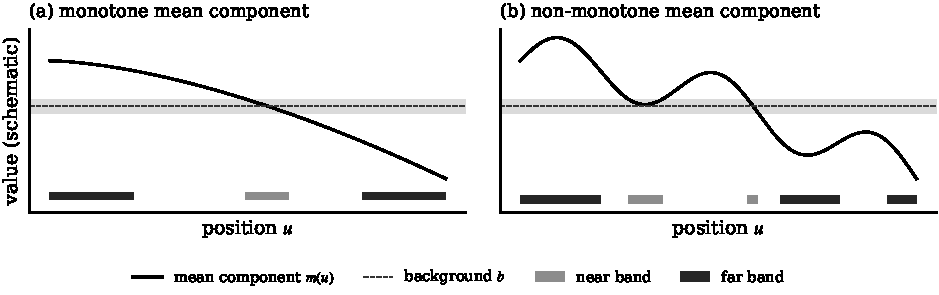
\includegraphics[width=\linewidth]{fig_state_bands.pdf}
\caption{Schematic of the state bands of A1 and A2 for an unconditional background $b$. (a) Monotone mean component: the near band and the far band of the mean component map onto intervals of positions. (b) Non-monotone mean component: the same bands map onto scattered positions.}
\label{fig:bands}
\end{figure}

\paragraph{Semantic artifacts.} \emph{A3, spurious-pattern response}: a substitute at the background's value inside a window whose mean component is far from it creates an abrupt departure and return, which resembles a localized pattern of the process. A model that has learned to respond to such patterns responds to the one that masking created. In the monotone instance, a substitute toward the background in a late window resembles a temporary recovery against the trend, the kind of localized pattern that DegradX inserts in its FORM profile \citep{degradx2026}. \emph{A4, directional offset}: masking pulls the model's reading of the window's mean component toward the background, so the signed change of the prediction depends on the sign of $b_c-m_{u,c}$. In the monotone instance, substituting late cells by mid-range values moves predictions toward earlier states.

\paragraph{Propagation artifacts.} \emph{A5, recurrent carry-over}: in a recurrent model, a substituted position alters the hidden state and therefore the processing of every later position, so the distortion is not confined to the masked cell. \emph{A6, coalition compounding}: Shapley values evaluate coalitions with many cells masked at once, so that A1--A5 act together within one model call.

\subsection{Ground truth per background, distortion and instruments}\label{sec:method:gt}

\paragraph{Ground truth.} Let $g$ be a known function that the trained model $f$ reproduces on the support of its training distribution. The ground truth for background $b$ is the Shapley value map of $g$ under the value function of $b$,
\begin{equation}\label{eq:gt}
\phi^\star_b := \phi\bigl(v^g_b\bigr), \qquad v^g_b(S) := g\bigl(\mask(x_W,S,b)\bigr).
\end{equation}
For an affine $g(x_W) = \beta_0 + \sum_{(u,c)\in W} w_{u,c}\,x_{u,c}$ and a coalition-independent $b$, the game $v^g_b$ is additive, and Equation~\eqref{eq:shapley} gives $\phi^\star_{b,u,c} = w_{u,c}\,(x_{u,c}-b_c(u;x))$ in closed form. Otherwise, $\phi^\star_b$ is computed by permutation sampling of $g$, which is cheap to evaluate, so its sampling error can be made negligible against the distortion and is reported.

\paragraph{Distortion.} The distortion of background $b$ is
\begin{equation}\label{eq:distortion}
D_b := A_b(f) - \phi^\star_b .
\end{equation}
Since the Shapley value is linear in the game \citep{sundararajan2020many}, $D_b$ is, up to estimation error, the Shapley value of the difference game
\begin{equation}\label{eq:diffgame}
\Delta_b(S) := v^f_b(S)-v^g_b(S) = f\bigl(\mask(x_W,S,b)\bigr)-g\bigl(\mask(x_W,S,b)\bigr).
\end{equation}
Since $f\approx g$ on the support, $\Delta_b$ nearly vanishes on every coalition whose substituted window stays on the support. $D_b$ therefore measures what the model's behaviour off its support contributes to the attribution, together with the residual misfit of $f$ on the support, which must therefore be small; $\phi^\star_b$ contains the information that the background removes. This separates the two parts named in the introduction. Under this definition no background is correct by construction, which removes the circularity for which DegradX declined trend-conditional backgrounds. The ground truth of every background is exact by construction, but its distortion vanishes only if its substituted windows keep $f$ on its support, which a coalition of many smooth, noise-free substitutes need not do (A6). $D_b$ is reported in target units as $\|D_b\|_1=\sum_{(u,c)}|D_{b,u,c}|$ and relative to $\|\phi^\star_b\|_1$, always beside $\EM_b$.

\paragraph{Ensemble divergence.} Equally accurate models $f_1,\dots,f_n$ that all reproduce $g$ on the support can differ in their attributions under $b$, beyond their residual misfit, only through their responses to substituted windows off the support. We introduce the \emph{ensemble divergence}
\begin{equation}\label{eq:ed}
\ED_b(x) := \sum_{(u,c)\in W} \operatorname{sd}_{k=1,\dots,n}\bigl(A_b(f_k)_{u,c}\bigr),
\end{equation}
the sum over cells of the across-model standard deviation, computed with the same coalition samples for every model. It measures how much an explanation depends on behaviour that no training data constrain, needs no ground truth, and therefore applies unchanged to models of measured data. It carries DegradX's ensemble range, the range of a score over ten equally accurate models \citep{degradx2026}, from scores to attribution maps.

\paragraph{Instruments.} One instrument is defined per artifact. Each is computed under every background, so that RQ1 reads its value under the unconditional backgrounds and RQ2 its paired difference under the others.
\begin{itemize}
\item \emph{M1 (A1).} On channels to which $g$ gives zero weight, $\phi^\star_b=0$ and $D_b=A_b(f)$. M1 is the Spearman correlation between $|D_{b,u,c}|$ and $d_{u,c}$ over the cells of such channels, reported with the share of $\sum|A_b(f)|$ that falls on them. Ideal value: 0.
\item \emph{M2 (A2).} For windows that contain localized patterns at known cells, M2 is the difference in retrieval of those cells between windows whose state lies in the far band and windows in the near band. Retrieval is the average precision with which $|A_b(f)(x_W)-A_b(f)(\tilde x_W)|$ ranks the pattern cells, $\tilde x_W$ being the pattern-free counterpart of the window \citep{degradx2026}. Ideal value: 0.
\item \emph{M3 (A3).} Under a target variable that depends only on the localized patterns that the generator inserts, the target is zero on every window without a pattern. Substitution does not insert patterns, so the ground truth of such a window is zero under every background. M3 is the attribution mass $\sum|A_b(f)|$ on such windows. Ideal value: 0.
\item \emph{M4 (A4).} The signed value-function distortion $\Delta_b(S)$, over the coalitions that the estimator evaluates, as a function of the state; reported as the slope and intercept of its regression on the state. Ideal values: 0 and 0. Without a known function, M4 is the centring of $f(\mask(x_W,S,b))-f(x_W)$ within strata of the state index. If the substitute is unbiased for the masked value at the window's state, this shift is centred on zero to first order in $f$, so a systematic sign identifies a biased background.
\item \emph{M5 (A5).} For a position $u_0$ substituted on all channels, $\tilde x^{(u_0)}_W$ denotes the window after substitution. M5 is the change this causes in the distortion at the other positions, $\mathrm{M5}(\ell) := \mathbb{E}\sum_c \bigl|D_b(\tilde x^{(u_0)}_W)_{u_0+\ell,c}-D_b(x_W)_{u_0+\ell,c}\bigr|$, as a function of the offset $\ell\neq 0$, compared between a recurrent model and a non-recurrent control. For an affine $g$, the ground truth at $u\neq u_0$ does not change, so carry-over appears as an excess of M5 at $\ell>0$ over $\ell<0$ in the recurrent model that the control does not show.
\item \emph{M6 (A6).} $|\Delta_b(S)|$ as a function of the number of masked cells $|W\setminus S|$, against the sum of the single-cell distortions $\sum_{i\in W\setminus S}|\Delta_b(W\setminus\{i\})|$. Growth above that sum is compounding.
\end{itemize}
The scores of DegradX, namely rank agreement, channel allocation error and temporal profile error, are computed for $A_b(f)$ against $\phi^\star_b$ as supporting measures \citep{degradx2026}.

\subsection{Backgrounds}\label{sec:method:backgrounds}

Table~\ref{tab:explained} lists the backgrounds by the quantity each one explains, following Equation~\eqref{eq:efficiency}. Figure~\ref{fig:toy} shows the substitutes of four of them on one window, together with the quantity each explains on an affine function.

\begin{table}[t]
\caption{What each background explains. Second column: the window on which $f$ is evaluated when all cells are masked; third: the sum of the attributions (Equation~\ref{eq:efficiency}).}
\label{tab:explained}
\centering
\small
\begin{tabularx}{\linewidth}{@{}>{\raggedright\arraybackslash}p{2.6cm}>{\raggedright\arraybackslash}p{3.2cm}>{\raggedright\arraybackslash}p{3.0cm}>{\raggedright\arraybackslash}X@{}}
\toprule
Background & All cells masked: $f$ evaluated on & Attributions sum to & Question answered \\
\midrule
B0, B1, B-pristine (unconditional) & a constant window $b$ & $f(x_W)-f(b)$ & Why does this prediction differ from a fixed reference? \\
B2, TAB-state (fine bins) & the population at this window's states & $f(x_W)-f(b_{\mathrm{state}}(x))$ & Why does it differ from a typical unit at the same state? \\
B3, TAB-traj & the extrapolation of the unit's own mean component & $f(x_W)-f(b_{\mathrm{traj}}(x))$ & What do the observations add beyond the unit's own past? \\
B2c, B4 (coalition-dependent) & the population marginal & $f(x_W)-f(b_1)$, B4 approximately & The B1 question, with coalitions that stay on the data support \\
\bottomrule
\end{tabularx}
\end{table}

\begin{figure}[t]
\centering
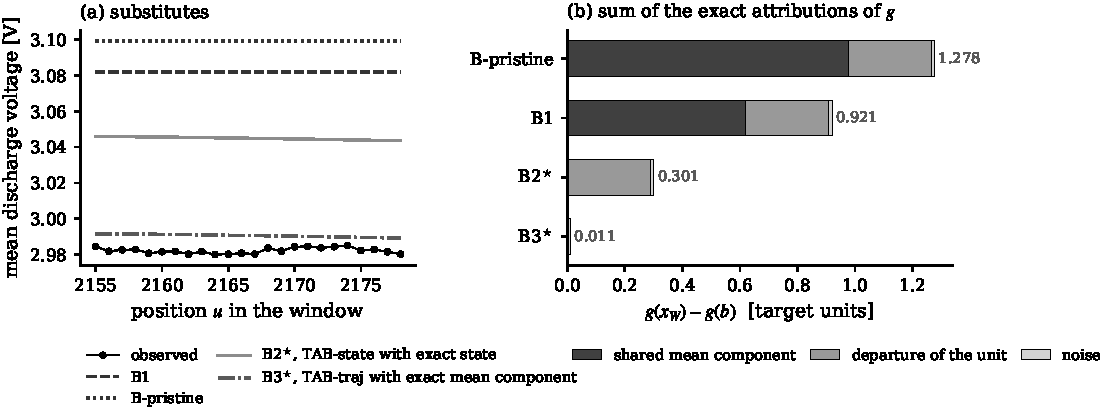
\includegraphics[width=\linewidth]{fig_toy_window.pdf}
\caption{One window ($L:=24$) of a unit generated by DegradX's HUST profile, the evaluation window with the largest final degradation state among the profile's 120 \citep{degradx2026}. (a) Observed mean discharge voltage and the substitute of each background; B2$^\star$ and B3$^\star$ are TAB-state and TAB-traj with the exact state and the unit's exact mean component. (b) Sum of the exact attributions of DegradX's affine reference model under each background, split into the parts due to the mean component shared by the units of the profile, the unit's departure from it, and the noise.}
\label{fig:toy}
\end{figure}

\paragraph{B0, B1 and B-pristine.} Attributions are computed in raw input space: the model is wrapped with its input standardization, so that every background is specified in the units of the data. Zero after standardization is the training mean, that is, B1; \emph{B0} is therefore zero in raw units, a floor reference. \emph{B1} is the per-channel mean over all positions of the training units, \dec{D3}{as in the authors' earlier study\todo{Verify against ACIIDS Eq.~3 (paper not available)}; TimeSHAP's average event, which its implementation computes as the per-channel median \citep{bento2021timeshap}, is reported as a variant}. \emph{B-pristine} places the pristine reference point of DegradX at every position; it is DegradX's primary baseline \citep{degradx2026}.

\paragraph{B2, TAB-state.} TAB-state substitutes the population mean of the channel among training observations at the same state. The state index of Equation~\eqref{eq:stateindex} is partitioned into $K$ bins $Q_1,\dots,Q_K$ by quantiles over the training units. With $k(u;x)$ the bin of $h_u(x)$,
\begin{equation}\label{eq:tabstate}
b^{\mathrm{state}}_c(u;x) := \frac{\sum_{j}\sum_{v}\mathbf{1}\{h_v(x_j)\in Q_{k(u;x)}\}\,x_{j,v,c}}{\sum_{j}\sum_{v}\mathbf{1}\{h_v(x_j)\in Q_{k(u;x)}\}},
\end{equation}
where $j$ runs over training units and $v$ over their positions. $b^{\mathrm{state}}$ is the binned estimate of the state-conditional expectation $\mathbb{E}[x_{v,c}\mid h_v\in Q_k]$, which replaces the unconditional expectation of B1. The index is computed from $x_{1:u-1}$ rather than $x_{1:u}$ for the reason given below for TAB-traj: otherwise the masked value would feed its own substitute. Bins below a minimum count are merged with their neighbour along the index. When several channels are mean-nonstationary, the coordinates of $h$ are selected on the training split: each channel's causal running summary is scored by its association with elapsed position within units, near-duplicates of a higher-scoring summary are removed, and the best remaining summaries are kept up to the cap $d$. A robust variant replaces the bin mean by the bin median. The table of bin means is computed once, and each substitute is a lookup.

$K$ changes the question, not only the balance between bias and variance. With $K=1$, $b^{\mathrm{state}}$ equals B1 and keeps the mean component in what is explained. As $K$ grows, the substitute approaches the population's mean component at the window's state, and the attributions sum to what distinguishes the unit from a typical unit at that state: its offsets, its localized patterns and its noise.

TAB-state assumes that (S1) conditioning on $h$ reduces the spread of $x_{u,c}$, diagnosed by the within-bin variance as a fraction of the total; (S2) units share one law of observation given the state, although they may differ in pace, diagnosed by the dispersion between units within a bin; (S3) every visited bin holds enough training observations, reported as the occupancy of the bins, with extreme states the most exposed; and (S4) $h$ is computable from $x_{1:u-1}$ without the target variable (R1). It assumes no shape of the mean component and needs no history of the unit beyond the short window of $h$. It blurs across fast changes of the mean component, treats two units at the same state alike, and coarsens when the law of observation depends on the path beyond the state.

\paragraph{B3, TAB-traj.} TAB-traj substitutes the one-step extrapolation of the unit's own mean component, fitted on its strict past. For channel $c$ and position $u$ with $u-1\ge t_{\min}$,
\begin{equation}\label{eq:tabtraj}
\hat m^{(u)}_c := \arg\min_{m\in\mathcal{M}} \sum_{v=1}^{u-1}\omega(u-v)\bigl(x_{v,c}-m(v)\bigr)^2 + \lambda P(m),
\qquad b^{\mathrm{traj}}_c(u;x) := \hat m^{(u)}_c(u),
\end{equation}
with a family $\mathcal{M}$ of smooth functions able to express sharp local curvature, a weight profile $\omega$, a roughness penalty $P$ and its weight $\lambda$, selected by cross-validation over training units. Below $t_{\min}$, TAB-traj falls back to TAB-state at the same position. The fit uses positions up to $u-1$ for two reasons. Including $x_{u,c}$ would make the substitute a smoothed copy of the value that masking is meant to remove, an under-perturbation that blunts the method by construction. Under the working decomposition $x_{v,c}=m(v)+\eta_v$ with $\mathbb{E}[\eta_v\mid x_{1:v-1}]=0$, the strict-past fit estimates $\mathbb{E}[x_{u,c}\mid x_{1:u-1}]$, so masking removes exactly the part of the observation that its own past does not predict. The fits are computed once per unit, channel and position and reused across coalitions.

TAB-traj assumes that (T1) the decomposition above holds, diagnosed by the autocorrelation and the mean of the fit residuals; (T2) $\mathcal{M}$ can express the curvature present, diagnosed by the fit residuals stratified by position, since a spike in them marks a substitute that may itself lie off the support; (T3) the strict past is long enough and informative about $u$, with no unannounced change at $u$; and (T4) the noise is small relative to the movement of the mean component, otherwise the fit's variance enters the substitute. It needs no population of units. Its cost is a shift in meaning: a cell that only confirms the unit's predictable course receives little attribution even if the model depends heavily on the mean component that the cell carries. This answers a different question from that of an analyst who asks how much the mean component at that cell matters.

Both TAB backgrounds therefore shift what is explained (Table~\ref{tab:explained}). With fine bins, TAB-state removes the population's mean component and explains the unit's departures from it; TAB-traj removes the unit's own mean component and explains what its past does not predict.

\paragraph{Oracles B2$^\star$ and B3$^\star$.} On generated units, where the state and the mean component are known exactly, two oracle backgrounds replace the estimates by the exact quantities. B2$^\star$ is the mean component shared by the units at the exact state, which TAB-state approaches with a perfect index and fine bins; B3$^\star$ is the unit's exact mean component, which TAB-traj approaches with a perfect fit. They bound what TAB can reach, and the gap from B2 to B2$^\star$ is the estimation error of the state index. Their explained quantities are those of TAB-state with fine bins and of TAB-traj (Table~\ref{tab:explained}). Figure~\ref{fig:tabs} contrasts the two on one unit.

\begin{figure}[t]
\centering
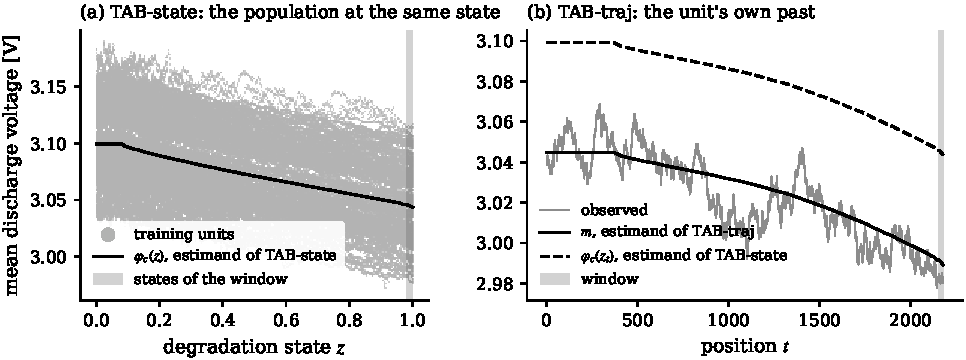
\includegraphics[width=\linewidth]{fig_tab_state_traj.pdf}
\caption{TAB-state against TAB-traj at their exact estimands, for the unit and channel of Figure~\ref{fig:toy}. (a) The channel over all training units of the profile against their exact degradation state, with the mapping $\varphi_c(z)$ shared by the units \citep{degradx2026}, the estimand of TAB-state; the band marks the states of the window. (b) The channel of the unit over its life, with its own mean component $m$, the estimand of TAB-traj, and $\varphi_c(z_t)$; the shaded positions are the window.}
\label{fig:tabs}
\end{figure}

\paragraph{B2c, coalition-conditional TAB.} \dec{D1}{B2c, a variant of TAB-state, keeps B1's explained quantity while keeping the coalitions near the window's own mean component. Each masked cell takes the mean of the retained cells of the same channel in the window; a channel masked entirely takes the training mean $b_{1,c}$,
\begin{equation}\label{eq:b2c}
b^{\mathrm{2c}}_c(u;S) := \begin{cases}
\frac{1}{|S_c|}\sum_{(v,c)\in S_c} x_{v,c}, & S_c\neq\emptyset,\\
b_{1,c}, & S_c=\emptyset,
\end{cases}\qquad S_c := \{(v,c')\in S : c'=c\}.
\end{equation}
When all cells are masked, the window equals that of B1, so the attributions sum to $f(x_W)-f(b_1)$. B2c depends on the coalition and is therefore not covered by (R2); it assumes that the mean component changes little within a window, and where it does change, the substitute is the window's average rather than the mean component at the masked position.}

\paragraph{B4, learned conditional imputer.} B4 is the generative on-manifold remedy of the Shapley literature \citep{frye2021shapley}, instantiated for windows. It is an established reference, not a contribution, and is not assumed to dominate. An imputer trained on unmasked training windows fills the masked cells with their conditional mean given the retained ones; with no cell retained, the fill is the population mean, so B4 approximately keeps B1's explained quantity. B4 depends on the coalition and requires one imputer call per coalition. Since the imputer is a second model whose misfit enters the substitute, its error on held-out masked cells is reported with every B4 result.

\paragraph{Choosing a background.} The two TAB backgrounds condition at different resolutions, and their weaknesses are largely complementary. Table~\ref{tab:guide} states the resulting guide; each row is a hypothesis.

\begin{table}[t]
\caption{Selection guide. Each row is a hypothesis.}
\label{tab:guide}
\centering
\small
\begin{tabularx}{\linewidth}{@{}>{\raggedright\arraybackslash}p{5.4cm}>{\raggedright\arraybackslash}p{2.6cm}>{\raggedright\arraybackslash}X@{}}
\toprule
Property of the data or question & Favours & Reason \\
\midrule
Many training units; short explained histories & TAB-state & bins are populated; TAB-traj unavailable below $t_{\min}$ \\
Single unit or a fleet without history & TAB-traj & needs no population \\
High noise in a channel & TAB-state & population averaging removes fit variance (T4) \\
Long histories; mean components that differ between units & TAB-traj & pooling would blur differences between units \\
Localized patterns present and used by the model & TAB-traj & conditioning on the unit removes the manufactured pattern (A3) \\
Sharp changes of the mean component & neither clearly & TAB-state blurs across the change; TAB-traj lags behind it \\
Same state, different course (path dependence) & TAB-traj & the state alone does not determine the observation \\
Does the absolute mean component here matter? & B1, B-pristine, B2c or B4 & only these keep the mean component in what is explained \\
\bottomrule
\end{tabularx}
\end{table}

\subsection{Evaluation design on DegradX}\label{sec:method:design}

Figure~\ref{fig:design} shows how the parts of the evaluation connect. Its synthetic arms use DegradX v1 as published, with extensions declared below; its measured arms and the case study use the same instruments without ground truth.

\begin{figure}[t]
\centering
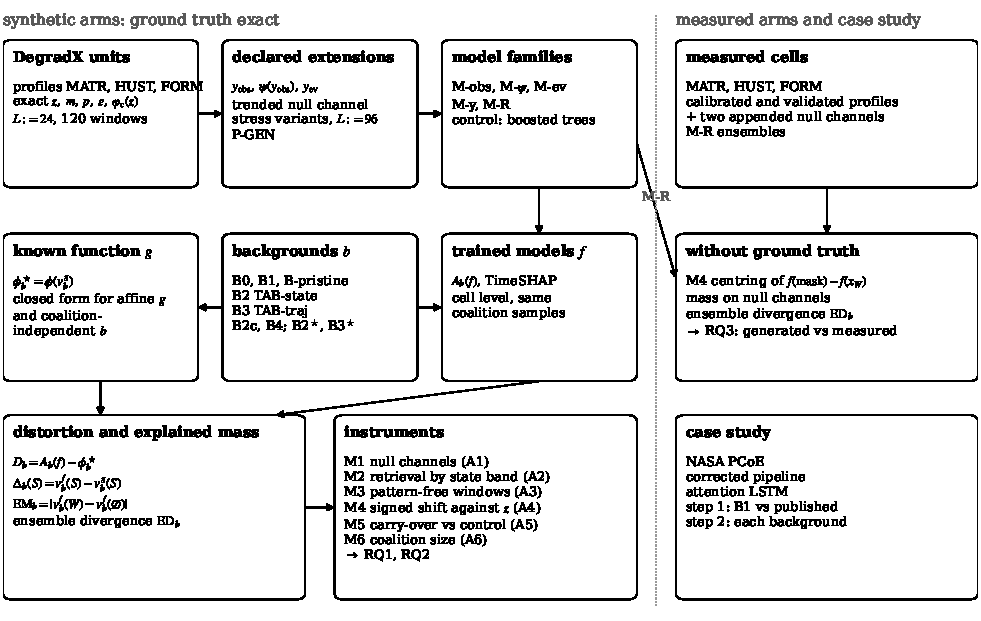
\includegraphics[width=\linewidth]{fig_eval_design.pdf}
\caption{Evaluation design. Generated units of the three DegradX profiles train the model families; each background yields a ground truth $\phi^\star_b$ on the known function and a distortion $D_b$ on the trained models, read through the instruments M1--M6 beside the explained mass. Measured cells and the case study are read with the instruments that need no ground truth.}
\label{fig:design}
\end{figure}

\paragraph{DegradX as used.} A generated unit of DegradX consists of channels $x_{t,c} = m_{t,c}+\sum_k p_{k,t,c}+\varepsilon_{t,c}$, the sum of a mean component, inserted patterns and noise, with $m_{t,c}=\varphi_c(z_t)+\delta_{c,i}$, where $z_t$ is the degradation state, $\varphi_c$ a monotone mapping shared by the units of a profile and $\delta_{c,i}$ a per-unit offset \citep{degradx2026}. The profiles MATR, HUST and FORM, their generator and seeds, and the exact decomposition of every unit are used unchanged: $z$, $m$, $p$, $\varepsilon$, and $\varphi_c(z)$ without offsets, which the repository records for every unit \citep{degradxrepo}. So are the reference model
\begin{equation}\label{eq:refmodel}
g(x_W) := \sum_{(u,c)\in W} w_{u,c}\,\bigl(x_{u,c}-x^0_c\bigr), \qquad x^0_c := \varphi_c(0),
\end{equation}
with weights $w_{u,c}=\kappa_c\pi_u$ under DegradX's recency profile $\pi_u\propto 2^{-(t-u)/h}$, $h:=L/4$; the two null channels, which do not depend on the degradation state, and DegradX's checks that a model does not use them; the ten-member LSTM ensembles of hidden size 64 with two layers and hidden size 128 with one layer, five initializations each \citep{degradxrepo}; the scores; the TSTR ratio of each profile; and the 120 evaluation windows of each profile \citep{degradx2026}. Models use the 300 units of generation seed 0, 210 for training, 45 for validation and 45 for testing \citep{degradx2026}. On DegradX, B-pristine is $x^0_c$ at every position, and the oracles are B2$^\star_c(u) := \varphi_c(z_u)$ and B3$^\star_c(u) := m_{u,c}$.

\paragraph{What DegradX's results imply.} Three results of DegradX determine the design. First, equally accurate models disagree more than methods do; in FORM, each method's range in rank agreement over the ten models is 0.32 to 0.34 \citep{degradx2026}. Scores against the common ground truth on models trained on $y$ therefore cannot rank backgrounds, which is why each background receives its own ground truth on a model with a known function. Second, a zero-weight channel that carries the degradation state cannot serve as a trap channel, that is, a channel that is mean-nonstationary but does not enter the target and whose correct attribution is therefore zero. In MATR, whose zero-weight channels internal resistance and temperature carry the state, the share of attribution on zero-weight channels is 0.134 to 0.198, against at most 0.048 in HUST and FORM, whose zero-weight channels are the null channels \citep{degradx2026}. A channel that carries the state predicts the target, so a model may legitimately use it, and its correct attribution is not zero. A trap channel must therefore be independent of the unit's state. Third, the inserted patterns of FORM carry $1.7\times10^{-5}$ of the variance of the mean term, and removing them from the target leaves the error of trained models unchanged \citep{degradx2026}. A model trained on $y$ has no reason to respond to them, so A3 requires a target driven by the patterns alone.

\paragraph{Declared extensions.} DegradX is not modified; this paper adds the following on top of it, each labelled where its results appear.
\begin{itemize}
\item \emph{Two target variables.} The observation-level target $y_{\mathrm{obs}} := g(x_W)$, the reference model applied to the observed window, noise included; and, \dec{D5}{conditional on the pilot}, $\psi(y_{\mathrm{obs}})$ for a monotone nonlinear $\psi$.
\item \emph{A trended null channel.} The degradation-state trajectory of another generated unit, read from a random starting position, held at its end-of-life value after that unit's record ends, mapped through the profile's charge-time mapping and given noise of the charge-time variance and autocorrelation. It has zero target weight, and it is accepted only if it passes DegradX's null-channel check and its conditional channel-use check on every model.
\item \emph{An event-driven target on FORM.} $y_{\mathrm{ev}} := \sum_{(u,c)\in W} w_{u,c}\sum_k p_{k,u,c}$, the sparse part of DegradX's target alone. Its ground truth on windows without patterns is zero everywhere.
\item \emph{Stress variants}, made with DegradX's existing generator overrides at the values of its declared grids: transition sharpness $z\mapsto z^s$, $s\in\{0.25,0.5,1,2,4\}$; noise-variance multiplier $\in\{0.25,0.5,1,2,4,8,16\}$; and pattern-amplitude multiplier $\in\{0.25,0.5,1,2,4,8\}$ \citep{degradxrepo}. They are not calibrated to any dataset.
\item \emph{One longer window}, $L:=$\,\dec{D2}{96} from DegradX's declared grid of window lengths \citep{degradxrepo},\todo{D2: use the ACIIDS sequence length if the ACIIDS paper states one (paper not available)} for A5 and for profiles of attribution within a window.
\item \emph{A non-monotone probe}, P-GEN: a slow periodic component added to the mean component of the weighted channels, so that the mean component is not monotone in position. DegradX's generator is monotone by construction, so P-GEN requires new generator code. Under $y_{\mathrm{obs}}$ the periodic component enters the target variable. P-GEN is not calibrated.
\end{itemize}

\paragraph{Model families.} All models are \dec{D7}{DegradX's LSTM regressor}, trained with DegradX's procedure in ten-member ensembles of the two architectures above \citep{degradxrepo}, except the control.
\begin{itemize}
\item \emph{M-obs}, trained on $y_{\mathrm{obs}}$, the primary family. Because $y_{\mathrm{obs}}$ is a deterministic function of the input window, a model that fits it reproduces $g$ on the support. A function-identity check confirms this for every member: on the windows of held-out generated units, the root-mean-square difference between $f$ and $g$ must lie within a fraction \dec{D8}{$\vartheta$} of the standard deviation of $\sum w\varepsilon$, the part of $y_{\mathrm{obs}}$ that a model of $y$ could not predict. Accuracy alone does not establish this: DegradX's ten equally accurate models need not learn the function that defines its ground truth, since the channels of a window share one degradation state and other functions reproduce the target equally well \citep{degradx2026}.
\item \emph{M-$\psi$}, trained on $\psi(y_{\mathrm{obs}})$, \dec{D5}{conditional on the pilot}. It covers the possibility that an LSTM fitted to an affine function stays nearly linear off its support, which would make every distortion small. Its ground truth is the Shapley value of $\psi\circ g$, computed by permutation sampling.
\item \emph{M-ev}, trained on $y_{\mathrm{ev}}$ on FORM, for M3.
\item \emph{M-y}, DegradX's released ensembles trained on $y$, read only with instruments that need no ground truth.
\item \emph{M-R}, trained on the RUL target $R$ of DegradX \citep{degradx2026}. Its inputs are the channels plus elapsed position, which is unmasked context rather than a player, since masking age with a fleet mean would be an A1 case of its own and would dominate. M-R ensembles are trained both on generated units and on measured cells.
\item \emph{The control}, gradient-boosted regression trees \citep{friedman2001greedy} on flattened windows, trained on $y_{\mathrm{obs}}$ at the longer $L$ together with an M-obs ensemble at that $L$; having no recurrent state, it is the non-recurrent control of M5.
\end{itemize}
For M-obs and every coalition-independent background, the ground truth is $\phi^\star_{b,u,c} = w_{u,c}(x_{u,c}-b_c(u;x))$; for B2c, B4 and M-$\psi$ it is computed by permutation sampling of the known function. The verdict on RQ1 and RQ2 rests on $D_b$ on M-obs, reported with $\EM_b$, as paired contrasts within models together with the number of members that agree in sign.

\paragraph{Instruments on DegradX.} Table~\ref{tab:instruments} gives the realization of each instrument. Ensemble divergence, explained mass and DegradX's scores against $\phi^\star_b$ are computed on every arm where they are defined.

\begin{table}[t]
\caption{Realization of the instruments on DegradX. $z$: exact degradation state.}
\label{tab:instruments}
\centering
\small
\begin{tabularx}{\linewidth}{@{}l>{\raggedright\arraybackslash}X>{\raggedright\arraybackslash}p{2.7cm}@{}}
\toprule
Artifact & Instrument & Models \\
\midrule
A1 & M1 on the two null channels and the trended null channel & M-obs, M-$\psi$; M-y, M-R on null channels \\
A2 & M2 on FORM, whose inserted patterns enter $y_{\mathrm{obs}}$ linearly; bands set by $z$ & M-obs (FORM) \\
A3 & M3 on windows without patterns, ground truth 0 & M-ev (FORM) \\
A4 & M4 against $z$: $f(\mask(x_W,S,b))-g(\mask(x_W,S,b))$; without $g$, centring of $f(\mask(x_W,S,b))-f(x_W)$ & all; centring only for M-y, M-R \\
A5 & M5 at $L:=96$, LSTM against the control & M-obs, control \\
A6 & M6 over the coalitions evaluated by the estimator & M-obs, M-$\psi$ \\
\bottomrule
\end{tabularx}
\end{table}

\paragraph{Operating envelope.} Five predictions test the selection guide on existing arms. (E1) TAB-traj's advantage over TAB-state grows with the available history and vanishes below $t_{\min}$, where the two coincide; read from $D_b$ stratified by $u-1$. (E2) TAB-state's advantage over B1 grows with the number of training units per bin; read from HUST against FORM on the measured arms, whose fitting splits hold 54 and 127 cells \citep{degradx2026}, and from nested random subsets of the generated training units, for which only the table of Equation~\eqref{eq:tabstate} is recomputed. (E3) Both TAB backgrounds degrade under sharp transitions, TAB-state by blur and TAB-traj by lag, distinguished by the fit residuals of (T2); read on the transition-sharpness variants. (E4) TAB-traj degrades faster than TAB-state as the noise variance grows; read on the noise-variance variants. (E5) TAB-state's correction shrinks more than TAB-traj's when the state no longer identifies the position; read on P-GEN. A falsified prediction corrects the guide.

\paragraph{Statistics.} Backgrounds are compared as paired contrasts within a model: on the same windows and with the same coalition samples of the estimator. Scores are averaged over the windows of a unit and then over units, and intervals are 95\% bootstrap intervals over units, as in DegradX, with 10{,}000 bias-corrected and accelerated resamples \citep{degradx2026, degradxrepo}. Each contrast is reported with the number of the ten members whose contrast has the same sign. Instruments are stratified by the exact degradation state on generated units and by the state index on measured cells.

\subsection{Measured data and case study}\label{sec:method:measured}

\paragraph{Measured arms.} The measured arms use the cells of MATR \citep{severson2019data}, HUST \citep{ma2022real} and FORM \citep{cui2024data}, each with its calibrated and validated DegradX profile. The TSTR ratio of each profile states how far its synthetic arm stands for the dataset: 1.17 [0.94, 1.34] for HUST, whose interval contains one, and 1.49 [1.04, 2.29] and 1.54 [1.28, 1.74] for MATR and FORM, which reproduce part, but not all, of the dependence between the sequences and the RUL \citep{degradx2026}. M-R ensembles trained on the fitting-split cells are read with the instruments that need no ground truth: the centring of M4, the attribution mass on null channels, and ensemble divergence. Two null channels, constructed as DegradX constructs them for generated units, a constant plus noise with the autocorrelation of the capacity noise and the measured values of a channel permuted across units and positions \citep{degradx2026}, are appended to the measured cells, so that the measured arms also have channels of known irrelevance. B-pristine takes $x^0$ from the profile of the dataset. The same instruments are computed on M-obs, so that RQ3 can compare the signatures found there with those of M-R models trained on generated units and on measured cells of the same dataset. On measured data they can falsify a background, since a background that fails a necessary condition is biased, but cannot certify one; certification rests on the synthetic arms.

\paragraph{Case study.} The case study re-examines the authors' own published attribution findings on their own corrected pipeline \citep{mishchuk2026explaining}; it is not an audit of the literature, and no external reproduction is attempted. It uses the battery data set of the NASA Prognostics Center of Excellence (PCoE) \citep{saha2007battery}\todo{Cells and preprocessing from the ACIIDS paper (not available)} and the attention LSTM of the earlier study\todo{Architecture from the ACIIDS paper}, which appears only here. The pipeline is corrected so that normalization statistics are computed on training cells alone and no input depends on positions after the predicted one, the rules DegradX applies \citep{degradx2026}.\todo{State what the published pipeline did differently, from the ACIIDS paper} The study has two steps. Step~1 runs the corrected pipeline with the original background, B1, and compares the result with the published values, which isolates the effect of the correction. Step~2 runs the corrected pipeline with each background, which isolates the effect of the background. For each published finding\todo{List of published findings from the ACIIDS paper}, a table states whether it survives step~1, step~2, both or neither.

\subsection{Implementation}\label{sec:method:impl}

All attributions use TimeSHAP 1.0.4 at DegradX's declared settings: cell level, $\textit{nsamples}:=32{,}000$ and pruning off \citep{bento2021timeshap, degradxrepo}. Coalition-independent backgrounds are passed to TimeSHAP as a background sequence of the window's length, $L\times C$, which the TimeSHAP 1.0.4 kernel accepts as an alternative to a single background event; DegradX's wrapper tiles a single event over the window, and passing the sequence is its only change. B2c and B4 do not fit a single background, since their substitute depends on the coalition; they require a modified masking step in the kernel, which computes the substitute for each sampled coalition before the model is called. All backgrounds of a contrast share the coalition-sampling seed.

The findings are stated for TimeSHAP, but the argument for their generality covers every substitution-based Shapley estimator. Each such estimator computes attributions as weighted aggregations of differences of $v_b$, and the background enters only through $v_b$. A1--A4 are properties of single model calls on substituted inputs, so their existence, sign and structure are common to the family, whereas magnitudes depend on how an estimator weights coalition sizes, which interacts with A6. A5 is a property of the architecture. One synthetic arm, one profile under B0, B1 and B2, is therefore replicated with TSHAP, which computes SHAP values exactly for groups of time steps \citep{nguyen2025tshap}, and compared at the level of signatures: the sign of M1, the profile of M4 against the state, and the ranking of the backgrounds.\todo{TSHAP applicability to the LSTM regressor and to cell-level players not verified (v5.1 \S9)}


%==============================================================================================
\section{Examples of citations, figures, tables, references}
\label{sec:others}
\lipsum[8] \cite{kour2014real,kour2014fast} and see \cite{hadash2018estimate}.

The documentation for \verb+natbib+ may be found at
\begin{center}
  \url{http://mirrors.ctan.org/macros/latex/contrib/natbib/natnotes.pdf}
\end{center}
Of note is the command \verb+\citet+, which produces citations
appropriate for use in inline text.  For example,
\begin{verbatim}
   \citet{hasselmo} investigated\dots
\end{verbatim}
produces
\begin{quote}
  Hasselmo, et al.\ (1995) investigated\dots
\end{quote}

\begin{center}
  \url{https://www.ctan.org/pkg/booktabs}
\end{center}


\subsection{Figures}
\lipsum[10] 
See Figure \ref{fig:fig1}. Here is how you add footnotes. \footnote{Sample of the first footnote.}
\lipsum[11] 

\begin{figure}
  \centering
  \fbox{\rule[-.5cm]{4cm}{4cm} \rule[-.5cm]{4cm}{0cm}}
  \caption{Sample figure caption.}
  \label{fig:fig1}
\end{figure}

\subsection{Tables}
\lipsum[12]
See awesome Table~\ref{tab:table}.

\begin{table}
 \caption{Sample table title}
  \centering
  \begin{tabular}{lll}
    \toprule
    \multicolumn{2}{c}{Part}                   \\
    \cmidrule(r){1-2}
    Name     & Description     & Size ($\mu$m) \\
    \midrule
    Dendrite & Input terminal  & $\sim$100     \\
    Axon     & Output terminal & $\sim$10      \\
    Soma     & Cell body       & up to $10^6$  \\
    \bottomrule
  \end{tabular}
  \label{tab:table}
\end{table}

\subsection{Lists}
\begin{itemize}
\item Lorem ipsum dolor sit amet
\item consectetur adipiscing elit. 
\item Aliquam dignissim blandit est, in dictum tortor gravida eget. In ac rutrum magna.
\end{itemize}


\section{Conclusion}
Your conclusion here

\section*{Acknowledgments}
This was was supported in part by......

%Bibliography
\bibliographystyle{unsrtnat}  
\bibliography{references}  


\end{document}
